\documentclass{standalone}
\usepackage{tikz}
\usetikzlibrary{patterns}
\usetikzlibrary{positioning}
\usetikzlibrary{patterns, positioning}
\usetikzlibrary{shapes.misc}
\usepackage[outline]{contour}
\contourlength{1.5pt} 
\usetikzlibrary{calc}
        \usepackage{relsize}
        \tikzset{fontscale/.style = {font=\relsize{#1}}}

\begin{document}
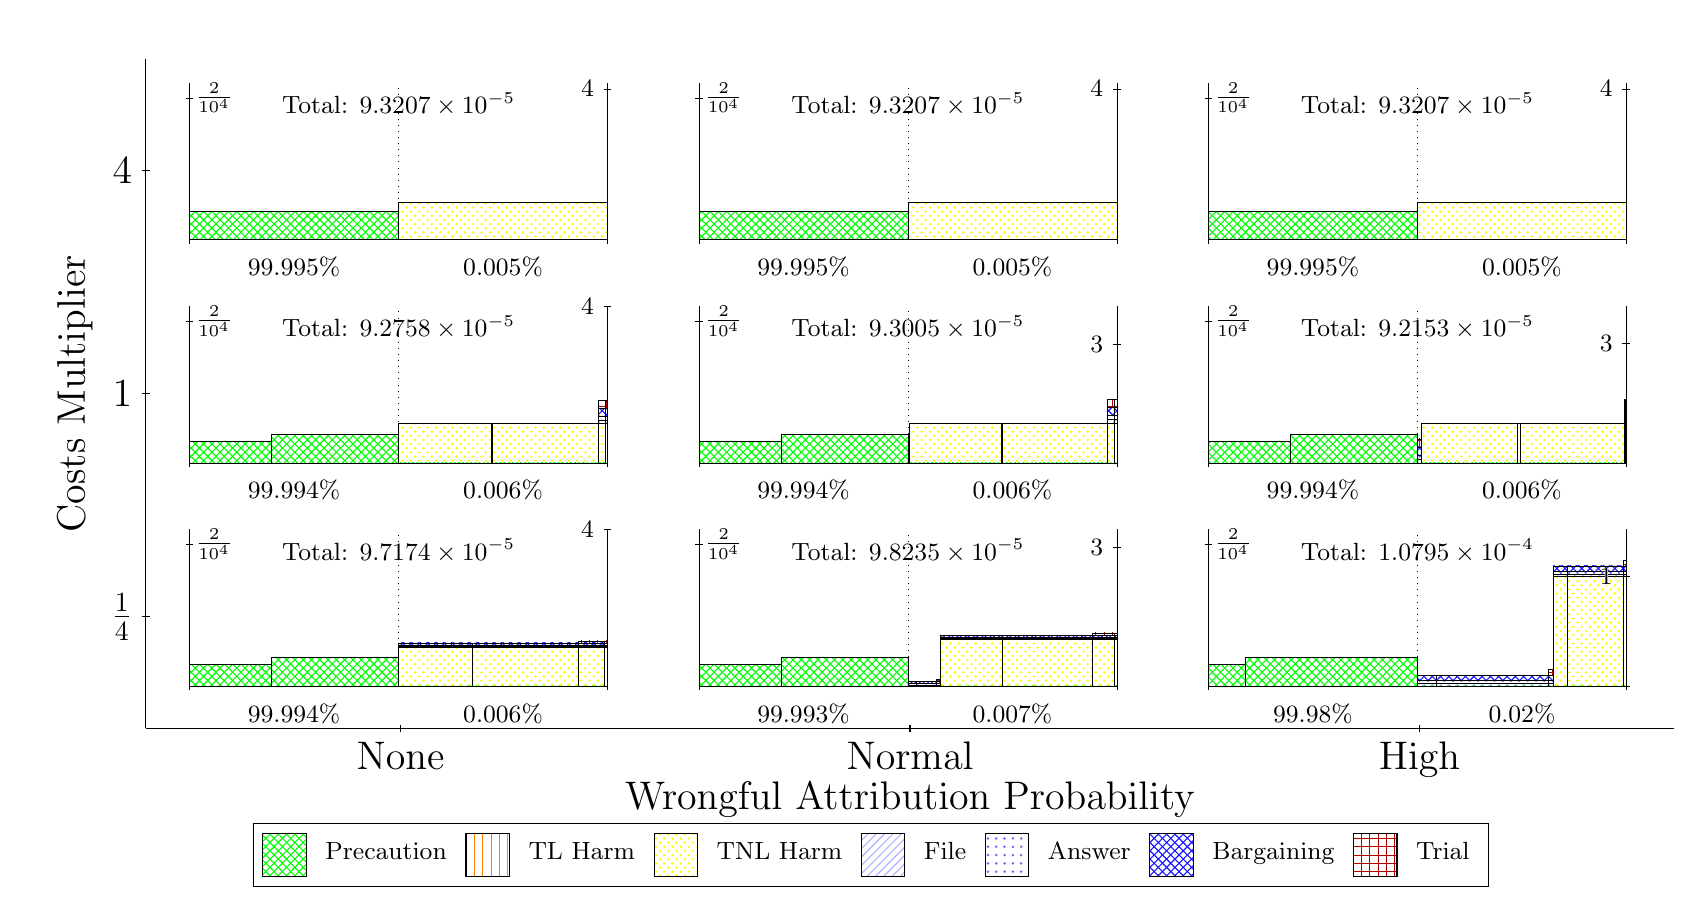
\begin{tikzpicture}
\clip(-0.5,-1.1) rectangle +(20.91,11);
\draw[black] (1,1) -- (1,9.5);
\node[rotate=90, fontscale=2, anchor=center] at (0.1, 5.25) {Costs Multiplier};
\draw[black] (0.95,2.4167) -- (1.05,2.4167);
\node[fontscale=2, anchor=east] at (0.95, 2.4167) {$\frac{1}{4}$};
\draw[black] (0.95,5.25) -- (1.05,5.25);
\node[fontscale=2, anchor=east] at (0.95, 5.25) {1};
\draw[black] (0.95,8.0833) -- (1.05,8.0833);
\node[fontscale=2, anchor=east] at (0.95, 8.0833) {4};

\draw[black] (1,1) -- (20.41,1);
\node[fontscale=2, anchor=center] at (10.705, 0.1) {Wrongful Attribution Probability};
\draw[black] (4.235,0.95) -- (4.235,1.05);
\node[fontscale=2, anchor=north] at (4.235, 0.95) {None};
\draw[black] (10.705,0.95) -- (10.705,1.05);
\node[fontscale=2, anchor=north] at (10.705, 0.95) {Normal};
\draw[black] (17.175,0.95) -- (17.175,1.05);
\node[fontscale=2, anchor=north] at (17.175, 0.95) {High};


\draw[pattern=crosshatch, pattern color=green,draw=black,very thin] (1.5556,1.54) rectangle (2.5958,1.8101);
\draw[pattern=crosshatch, pattern color=green,draw=black,very thin] (2.5958,1.54) rectangle (4.21,1.9002);
\draw[pattern=crosshatch, pattern color=green,draw=black,very thin] (4.21,1.54) rectangle (5.1455,1.54);
\draw[pattern=crosshatch dots, pattern color=yellow,draw=black,very thin] (4.21,1.54) rectangle (5.1455,2.037);
\draw[pattern=north east lines, pattern color=blue!30,draw=black,very thin] (4.21,2.037) rectangle (5.1455,2.0494);
\draw[pattern=dots,  pattern color=blue!60,draw=black,very thin] (4.21,2.0494) rectangle (5.1455,2.0618);
\draw[pattern=crosshatch,      pattern color=blue!90,draw=black,very thin] (4.21,2.0618) rectangle (5.1455,2.0867);
\draw[pattern=crosshatch, pattern color=green,draw=black,very thin] (5.1455,1.54) rectangle (5.1478,1.54);
\draw[pattern=vertical lines, pattern color=orange,draw=black,very thin] (5.1455,1.54) rectangle (5.1478,2.037);
\draw[pattern=north east lines, pattern color=blue!30,draw=black,very thin] (5.1455,2.037) rectangle (5.1478,2.0494);
\draw[pattern=dots,  pattern color=blue!60,draw=black,very thin] (5.1455,2.0494) rectangle (5.1478,2.0618);
\draw[pattern=crosshatch,      pattern color=blue!90,draw=black,very thin] (5.1455,2.0618) rectangle (5.1478,2.0867);
\draw[pattern=crosshatch, pattern color=green,draw=black,very thin] (5.1478,1.54) rectangle (6.4973,1.54);
\draw[pattern=crosshatch dots, pattern color=yellow,draw=black,very thin] (5.1478,1.54) rectangle (6.4973,2.037);
\draw[pattern=north east lines, pattern color=blue!30,draw=black,very thin] (5.1478,2.037) rectangle (6.4973,2.0494);
\draw[pattern=dots,  pattern color=blue!60,draw=black,very thin] (5.1478,2.0494) rectangle (6.4973,2.0618);
\draw[pattern=crosshatch,      pattern color=blue!90,draw=black,very thin] (5.1478,2.0618) rectangle (6.4973,2.0867);
\draw[pattern=crosshatch, pattern color=green,draw=black,very thin] (6.4973,1.54) rectangle (6.8237,1.54);
\draw[pattern=crosshatch dots, pattern color=yellow,draw=black,very thin] (6.4973,1.54) rectangle (6.8237,2.037);
\draw[pattern=north east lines, pattern color=blue!30,draw=black,very thin] (6.4973,2.037) rectangle (6.8237,2.0494);
\draw[pattern=dots,  pattern color=blue!60,draw=black,very thin] (6.4973,2.0494) rectangle (6.8237,2.0618);
\draw[pattern=crosshatch,      pattern color=blue!90,draw=black,very thin] (6.4973,2.0618) rectangle (6.8237,2.0867);
\draw[pattern=grid,            pattern color=red!70!black,draw=black,very thin] (6.4973,2.0867) rectangle (6.8237,2.1115);
\draw[pattern=crosshatch, pattern color=green,draw=black,very thin] (6.8237,1.54) rectangle (6.8644,1.54);
\draw[pattern=vertical lines, pattern color=orange,draw=black,very thin] (6.8237,1.54) rectangle (6.8644,2.037);
\draw[pattern=north east lines, pattern color=blue!30,draw=black,very thin] (6.8237,2.037) rectangle (6.8644,2.0494);
\draw[pattern=dots,  pattern color=blue!60,draw=black,very thin] (6.8237,2.0494) rectangle (6.8644,2.0618);
\draw[pattern=crosshatch,      pattern color=blue!90,draw=black,very thin] (6.8237,2.0618) rectangle (6.8644,2.0867);
\draw[pattern=grid,            pattern color=red!70!black,draw=black,very thin] (6.8237,2.0867) rectangle (6.8644,2.1115);
\node[font=\small,text=black,anchor=north] at (4.21, 3.5333) {Total: $9.7174\times 10^{-5}$};
\draw[black,very thin] (1.5556,1.54) -- (1.5556,3.5333);
\draw[black,very thin] (1.5056,3.3408) -- (1.6056,3.3408);
\node[font=\small,text=black, anchor=west] at (1.5056, 3.3408) {$\frac{2}{10^{4}}$};

\draw[black,dotted,very thin] (4.21,1.5998) -- (4.21,3.4735);
\draw[black,very thin] (6.8644,1.54) -- (6.8644,3.5333);
\draw[black,very thin] (6.8144,3.5279) -- (6.9144,3.5279);
\node[font=\small,text=black, anchor=east] at (6.8144, 3.5279) {\contour{white}{4}};

\draw[black,very thin] (1.5556,1.54) -- (6.8644,1.54);
\draw[black,very thin] (1.5556,1.49) -- (1.5556,1.59);
\node[font=\small,text=black, anchor=north] at (1.5556, 1.49) {};
\draw[black,very thin] (6.8644,1.49) -- (6.8644,1.59);
\node[font=\small,text=black, anchor=north] at (6.8644, 1.49) {};

\node[font=\small,text=black,anchor=south] at (2.8828, 0.94) {99.994\%};
\node[font=\small,text=black,anchor=south] at (5.5372, 0.94) {0.006\%};

\draw[pattern=crosshatch, pattern color=green,draw=black,very thin] (8.0256,1.54) rectangle (9.0658,1.8101);
\draw[pattern=crosshatch, pattern color=green,draw=black,very thin] (9.0658,1.54) rectangle (10.68,1.9001);
\draw[pattern=crosshatch, pattern color=green,draw=black,very thin] (10.68,1.54) rectangle (10.791,1.54);
\draw[pattern=north east lines, pattern color=blue!30,draw=black,very thin] (10.68,1.54) rectangle (10.791,1.5547);
\draw[pattern=dots,  pattern color=blue!60,draw=black,very thin] (10.68,1.5547) rectangle (10.791,1.5694);
\draw[pattern=crosshatch,      pattern color=blue!90,draw=black,very thin] (10.68,1.5694) rectangle (10.791,1.5987);
\draw[pattern=crosshatch, pattern color=green,draw=black,very thin] (10.791,1.54) rectangle (11.039,1.54);
\draw[pattern=north east lines, pattern color=blue!30,draw=black,very thin] (10.791,1.54) rectangle (11.039,1.5547);
\draw[pattern=dots,  pattern color=blue!60,draw=black,very thin] (10.791,1.5547) rectangle (11.039,1.5694);
\draw[pattern=crosshatch,      pattern color=blue!90,draw=black,very thin] (10.791,1.5694) rectangle (11.039,1.5987);
\draw[pattern=crosshatch, pattern color=green,draw=black,very thin] (11.039,1.54) rectangle (11.087,1.54);
\draw[pattern=north east lines, pattern color=blue!30,draw=black,very thin] (11.039,1.54) rectangle (11.087,1.5547);
\draw[pattern=dots,  pattern color=blue!60,draw=black,very thin] (11.039,1.5547) rectangle (11.087,1.5694);
\draw[pattern=crosshatch,      pattern color=blue!90,draw=black,very thin] (11.039,1.5694) rectangle (11.087,1.5987);
\draw[pattern=grid,            pattern color=red!70!black,draw=black,very thin] (11.039,1.5987) rectangle (11.087,1.6281);
\draw[pattern=crosshatch, pattern color=green,draw=black,very thin] (11.087,1.54) rectangle (11.879,1.54);
\draw[pattern=crosshatch dots, pattern color=yellow,draw=black,very thin] (11.087,1.54) rectangle (11.879,2.127);
\draw[pattern=north east lines, pattern color=blue!30,draw=black,very thin] (11.087,2.127) rectangle (11.879,2.1417);
\draw[pattern=dots,  pattern color=blue!60,draw=black,very thin] (11.087,2.1417) rectangle (11.879,2.1564);
\draw[pattern=crosshatch,      pattern color=blue!90,draw=black,very thin] (11.087,2.1564) rectangle (11.879,2.1857);
\draw[pattern=crosshatch, pattern color=green,draw=black,very thin] (11.879,1.54) rectangle (11.881,1.54);
\draw[pattern=vertical lines, pattern color=orange,draw=black,very thin] (11.879,1.54) rectangle (11.881,2.127);
\draw[pattern=north east lines, pattern color=blue!30,draw=black,very thin] (11.879,2.127) rectangle (11.881,2.1417);
\draw[pattern=dots,  pattern color=blue!60,draw=black,very thin] (11.879,2.1417) rectangle (11.881,2.1564);
\draw[pattern=crosshatch,      pattern color=blue!90,draw=black,very thin] (11.879,2.1564) rectangle (11.881,2.1857);
\draw[pattern=crosshatch, pattern color=green,draw=black,very thin] (11.881,1.54) rectangle (13.024,1.54);
\draw[pattern=crosshatch dots, pattern color=yellow,draw=black,very thin] (11.881,1.54) rectangle (13.024,2.127);
\draw[pattern=north east lines, pattern color=blue!30,draw=black,very thin] (11.881,2.127) rectangle (13.024,2.1417);
\draw[pattern=dots,  pattern color=blue!60,draw=black,very thin] (11.881,2.1417) rectangle (13.024,2.1564);
\draw[pattern=crosshatch,      pattern color=blue!90,draw=black,very thin] (11.881,2.1564) rectangle (13.024,2.1857);
\draw[pattern=crosshatch, pattern color=green,draw=black,very thin] (13.024,1.54) rectangle (13.3,1.54);
\draw[pattern=crosshatch dots, pattern color=yellow,draw=black,very thin] (13.024,1.54) rectangle (13.3,2.127);
\draw[pattern=north east lines, pattern color=blue!30,draw=black,very thin] (13.024,2.127) rectangle (13.3,2.1417);
\draw[pattern=dots,  pattern color=blue!60,draw=black,very thin] (13.024,2.1417) rectangle (13.3,2.1564);
\draw[pattern=crosshatch,      pattern color=blue!90,draw=black,very thin] (13.024,2.1564) rectangle (13.3,2.1857);
\draw[pattern=grid,            pattern color=red!70!black,draw=black,very thin] (13.024,2.1857) rectangle (13.3,2.2151);
\draw[pattern=crosshatch, pattern color=green,draw=black,very thin] (13.3,1.54) rectangle (13.334,1.54);
\draw[pattern=vertical lines, pattern color=orange,draw=black,very thin] (13.3,1.54) rectangle (13.334,2.127);
\draw[pattern=north east lines, pattern color=blue!30,draw=black,very thin] (13.3,2.127) rectangle (13.334,2.1417);
\draw[pattern=dots,  pattern color=blue!60,draw=black,very thin] (13.3,2.1417) rectangle (13.334,2.1564);
\draw[pattern=crosshatch,      pattern color=blue!90,draw=black,very thin] (13.3,2.1564) rectangle (13.334,2.1857);
\draw[pattern=grid,            pattern color=red!70!black,draw=black,very thin] (13.3,2.1857) rectangle (13.334,2.2151);
\node[font=\small,text=black,anchor=north] at (10.68, 3.5333) {Total: $9.8235\times 10^{-5}$};
\draw[black,very thin] (8.0256,1.54) -- (8.0256,3.5333);
\draw[black,very thin] (7.9756,3.3407) -- (8.0756,3.3407);
\node[font=\small,text=black, anchor=west] at (7.9756, 3.3407) {$\frac{2}{10^{4}}$};

\draw[black,dotted,very thin] (10.68,1.5998) -- (10.68,3.4735);
\draw[black,very thin] (13.334,1.54) -- (13.334,3.5333);
\draw[black,very thin] (13.284,3.301) -- (13.384,3.301);
\node[font=\small,text=black, anchor=east] at (13.284, 3.301) {\contour{white}{3}};

\draw[black,very thin] (8.0256,1.54) -- (13.334,1.54);
\draw[black,very thin] (8.0256,1.49) -- (8.0256,1.59);
\node[font=\small,text=black, anchor=north] at (8.0256, 1.49) {};
\draw[black,very thin] (13.334,1.49) -- (13.334,1.59);
\node[font=\small,text=black, anchor=north] at (13.334, 1.49) {};

\node[font=\small,text=black,anchor=south] at (9.3528, 0.94) {99.993\%};
\node[font=\small,text=black,anchor=south] at (12.007, 0.94) {0.007\%};

\draw[pattern=crosshatch, pattern color=green,draw=black,very thin] (14.496,1.54) rectangle (14.963,1.8101);
\draw[pattern=crosshatch, pattern color=green,draw=black,very thin] (14.963,1.54) rectangle (17.15,1.9001);
\draw[pattern=crosshatch, pattern color=green,draw=black,very thin] (17.15,1.54) rectangle (17.389,1.54);
\draw[pattern=north east lines, pattern color=blue!30,draw=black,very thin] (17.15,1.54) rectangle (17.389,1.5747);
\draw[pattern=dots,  pattern color=blue!60,draw=black,very thin] (17.15,1.5747) rectangle (17.389,1.6094);
\draw[pattern=crosshatch,      pattern color=blue!90,draw=black,very thin] (17.15,1.6094) rectangle (17.389,1.6787);
\draw[pattern=crosshatch, pattern color=green,draw=black,very thin] (17.389,1.54) rectangle (18.809,1.5401);
\draw[pattern=north east lines, pattern color=blue!30,draw=black,very thin] (17.389,1.5401) rectangle (18.809,1.5747);
\draw[pattern=dots,  pattern color=blue!60,draw=black,very thin] (17.389,1.5747) rectangle (18.809,1.6094);
\draw[pattern=crosshatch,      pattern color=blue!90,draw=black,very thin] (17.389,1.6094) rectangle (18.809,1.6787);
\draw[pattern=crosshatch, pattern color=green,draw=black,very thin] (18.809,1.54) rectangle (18.874,1.54);
\draw[pattern=north east lines, pattern color=blue!30,draw=black,very thin] (18.809,1.54) rectangle (18.874,1.5747);
\draw[pattern=dots,  pattern color=blue!60,draw=black,very thin] (18.809,1.5747) rectangle (18.874,1.6094);
\draw[pattern=crosshatch,      pattern color=blue!90,draw=black,very thin] (18.809,1.6094) rectangle (18.874,1.6787);
\draw[pattern=grid,            pattern color=red!70!black,draw=black,very thin] (18.809,1.6787) rectangle (18.874,1.748);
\draw[pattern=crosshatch, pattern color=green,draw=black,very thin] (18.874,1.54) rectangle (19.047,1.54);
\draw[pattern=crosshatch dots, pattern color=yellow,draw=black,very thin] (18.874,1.54) rectangle (19.047,2.9267);
\draw[pattern=north east lines, pattern color=blue!30,draw=black,very thin] (18.874,2.9267) rectangle (19.047,2.9613);
\draw[pattern=dots,  pattern color=blue!60,draw=black,very thin] (18.874,2.9613) rectangle (19.047,2.996);
\draw[pattern=crosshatch,      pattern color=blue!90,draw=black,very thin] (18.874,2.996) rectangle (19.047,3.0653);
\draw[pattern=crosshatch, pattern color=green,draw=black,very thin] (19.047,1.54) rectangle (19.761,1.5401);
\draw[pattern=crosshatch dots, pattern color=yellow,draw=black,very thin] (19.047,1.5401) rectangle (19.761,2.9267);
\draw[pattern=north east lines, pattern color=blue!30,draw=black,very thin] (19.047,2.9267) rectangle (19.761,2.9614);
\draw[pattern=dots,  pattern color=blue!60,draw=black,very thin] (19.047,2.9614) rectangle (19.761,2.996);
\draw[pattern=crosshatch,      pattern color=blue!90,draw=black,very thin] (19.047,2.996) rectangle (19.761,3.0653);
\draw[pattern=crosshatch, pattern color=green,draw=black,very thin] (19.761,1.54) rectangle (19.803,1.54);
\draw[pattern=crosshatch dots, pattern color=yellow,draw=black,very thin] (19.761,1.54) rectangle (19.803,2.9267);
\draw[pattern=north east lines, pattern color=blue!30,draw=black,very thin] (19.761,2.9267) rectangle (19.803,2.9613);
\draw[pattern=dots,  pattern color=blue!60,draw=black,very thin] (19.761,2.9613) rectangle (19.803,2.996);
\draw[pattern=crosshatch,      pattern color=blue!90,draw=black,very thin] (19.761,2.996) rectangle (19.803,3.0653);
\draw[pattern=grid,            pattern color=red!70!black,draw=black,very thin] (19.761,3.0653) rectangle (19.803,3.1347);
\draw[pattern=crosshatch, pattern color=green,draw=black,very thin] (19.803,1.54) rectangle (19.804,1.54);
\draw[pattern=vertical lines, pattern color=orange,draw=black,very thin] (19.803,1.54) rectangle (19.804,2.9267);
\draw[pattern=north east lines, pattern color=blue!30,draw=black,very thin] (19.803,2.9267) rectangle (19.804,2.9613);
\draw[pattern=dots,  pattern color=blue!60,draw=black,very thin] (19.803,2.9613) rectangle (19.804,2.996);
\draw[pattern=crosshatch,      pattern color=blue!90,draw=black,very thin] (19.803,2.996) rectangle (19.804,3.0653);
\draw[pattern=grid,            pattern color=red!70!black,draw=black,very thin] (19.803,3.0653) rectangle (19.804,3.1347);
\node[font=\small,text=black,anchor=north] at (17.15, 3.5333) {Total: $1.0795\times 10^{-4}$};
\draw[black,very thin] (14.496,1.54) -- (14.496,3.5333);
\draw[black,very thin] (14.446,3.3406) -- (14.546,3.3406);
\node[font=\small,text=black, anchor=west] at (14.446, 3.3406) {$\frac{2}{10^{4}}$};

\draw[black,dotted,very thin] (17.15,1.5998) -- (17.15,3.4735);
\draw[black,very thin] (19.804,1.54) -- (19.804,3.5333);
\draw[black,very thin] (19.754,1.54) -- (19.854,1.54);
\node[font=\small,text=black, anchor=east] at (19.754, 1.54) {\contour{white}{}};
\draw[black,very thin] (19.754,2.9266) -- (19.854,2.9266);
\node[font=\small,text=black, anchor=east] at (19.754, 2.9266) {\contour{white}{1}};

\draw[black,very thin] (14.496,1.54) -- (19.804,1.54);
\draw[black,very thin] (14.496,1.49) -- (14.496,1.59);
\node[font=\small,text=black, anchor=north] at (14.496, 1.49) {};
\draw[black,very thin] (19.804,1.49) -- (19.804,1.59);
\node[font=\small,text=black, anchor=north] at (19.804, 1.49) {};

\node[font=\small,text=black,anchor=south] at (15.823, 0.94) {99.98\%};
\node[font=\small,text=black,anchor=south] at (18.477, 0.94) {0.02\%};

\draw[pattern=crosshatch, pattern color=green,draw=black,very thin] (1.5556,4.3733) rectangle (2.5958,4.6434);
\draw[pattern=crosshatch, pattern color=green,draw=black,very thin] (2.5958,4.3733) rectangle (4.21,4.7335);
\draw[pattern=crosshatch, pattern color=green,draw=black,very thin] (4.21,4.3733) rectangle (5.3837,4.3733);
\draw[pattern=crosshatch dots, pattern color=yellow,draw=black,very thin] (4.21,4.3733) rectangle (5.3837,4.8703);
\draw[pattern=crosshatch, pattern color=green,draw=black,very thin] (5.3837,4.3733) rectangle (5.3959,4.3733);
\draw[pattern=vertical lines, pattern color=orange,draw=black,very thin] (5.3837,4.3733) rectangle (5.3959,4.8703);
\draw[pattern=crosshatch, pattern color=green,draw=black,very thin] (5.3959,4.3733) rectangle (6.7454,4.3734);
\draw[pattern=crosshatch dots, pattern color=yellow,draw=black,very thin] (5.3959,4.3734) rectangle (6.7454,4.8703);
\draw[pattern=crosshatch, pattern color=green,draw=black,very thin] (6.7454,4.3733) rectangle (6.8336,4.3733);
\draw[pattern=crosshatch dots, pattern color=yellow,draw=black,very thin] (6.7454,4.3733) rectangle (6.8336,4.8703);
\draw[pattern=north east lines, pattern color=blue!30,draw=black,very thin] (6.7454,4.8703) rectangle (6.8336,4.92);
\draw[pattern=dots,  pattern color=blue!60,draw=black,very thin] (6.7454,4.92) rectangle (6.8336,4.9697);
\draw[pattern=crosshatch,      pattern color=blue!90,draw=black,very thin] (6.7454,4.9697) rectangle (6.8336,5.0691);
\draw[pattern=grid,            pattern color=red!70!black,draw=black,very thin] (6.7454,5.0691) rectangle (6.8336,5.1685);
\draw[pattern=crosshatch, pattern color=green,draw=black,very thin] (6.8336,4.3733) rectangle (6.8644,4.3733);
\draw[pattern=vertical lines, pattern color=orange,draw=black,very thin] (6.8336,4.3733) rectangle (6.8644,4.8703);
\draw[pattern=north east lines, pattern color=blue!30,draw=black,very thin] (6.8336,4.8703) rectangle (6.8644,4.92);
\draw[pattern=dots,  pattern color=blue!60,draw=black,very thin] (6.8336,4.92) rectangle (6.8644,4.9697);
\draw[pattern=crosshatch,      pattern color=blue!90,draw=black,very thin] (6.8336,4.9697) rectangle (6.8644,5.0691);
\draw[pattern=grid,            pattern color=red!70!black,draw=black,very thin] (6.8336,5.0691) rectangle (6.8644,5.1685);
\node[font=\small,text=black,anchor=north] at (4.21, 6.3667) {Total: $9.2758\times 10^{-5}$};
\draw[black,very thin] (1.5556,4.3733) -- (1.5556,6.3667);
\draw[black,very thin] (1.5056,6.1741) -- (1.6056,6.1741);
\node[font=\small,text=black, anchor=west] at (1.5056, 6.1741) {$\frac{2}{10^{4}}$};

\draw[black,dotted,very thin] (4.21,4.4331) -- (4.21,6.3069);
\draw[black,very thin] (6.8644,4.3733) -- (6.8644,6.3667);
\draw[black,very thin] (6.8144,6.3612) -- (6.9144,6.3612);
\node[font=\small,text=black, anchor=east] at (6.8144, 6.3612) {\contour{white}{4}};

\draw[black,very thin] (1.5556,4.3733) -- (6.8644,4.3733);
\draw[black,very thin] (1.5556,4.3233) -- (1.5556,4.4233);
\node[font=\small,text=black, anchor=north] at (1.5556, 4.3233) {};
\draw[black,very thin] (6.8644,4.3233) -- (6.8644,4.4233);
\node[font=\small,text=black, anchor=north] at (6.8644, 4.3233) {};

\node[font=\small,text=black,anchor=south] at (2.8828, 3.7733) {99.994\%};
\node[font=\small,text=black,anchor=south] at (5.5372, 3.7733) {0.006\%};

\draw[pattern=crosshatch, pattern color=green,draw=black,very thin] (8.0256,4.3733) rectangle (9.0658,4.6434);
\draw[pattern=crosshatch, pattern color=green,draw=black,very thin] (9.0658,4.3733) rectangle (10.68,4.7335);
\draw[pattern=crosshatch, pattern color=green,draw=black,very thin] (10.68,4.3733) rectangle (10.7,4.3733);
\draw[pattern=north east lines, pattern color=blue!30,draw=black,very thin] (10.68,4.3733) rectangle (10.7,4.4234);
\draw[pattern=dots,  pattern color=blue!60,draw=black,very thin] (10.68,4.4234) rectangle (10.7,4.4735);
\draw[pattern=crosshatch,      pattern color=blue!90,draw=black,very thin] (10.68,4.4735) rectangle (10.7,4.5736);
\draw[pattern=grid,            pattern color=red!70!black,draw=black,very thin] (10.68,4.5736) rectangle (10.7,4.6738);
\draw[pattern=crosshatch, pattern color=green,draw=black,very thin] (10.7,4.3733) rectangle (11.865,4.3733);
\draw[pattern=crosshatch dots, pattern color=yellow,draw=black,very thin] (10.7,4.3733) rectangle (11.865,4.874);
\draw[pattern=crosshatch, pattern color=green,draw=black,very thin] (11.865,4.3733) rectangle (11.877,4.3733);
\draw[pattern=vertical lines, pattern color=orange,draw=black,very thin] (11.865,4.3733) rectangle (11.877,4.874);
\draw[pattern=crosshatch, pattern color=green,draw=black,very thin] (11.877,4.3733) rectangle (13.216,4.3734);
\draw[pattern=crosshatch dots, pattern color=yellow,draw=black,very thin] (11.877,4.3734) rectangle (13.216,4.874);
\draw[pattern=crosshatch, pattern color=green,draw=black,very thin] (13.216,4.3733) rectangle (13.304,4.3733);
\draw[pattern=crosshatch dots, pattern color=yellow,draw=black,very thin] (13.216,4.3733) rectangle (13.304,4.874);
\draw[pattern=north east lines, pattern color=blue!30,draw=black,very thin] (13.216,4.874) rectangle (13.304,4.9241);
\draw[pattern=dots,  pattern color=blue!60,draw=black,very thin] (13.216,4.9241) rectangle (13.304,4.9742);
\draw[pattern=crosshatch,      pattern color=blue!90,draw=black,very thin] (13.216,4.9742) rectangle (13.304,5.0743);
\draw[pattern=grid,            pattern color=red!70!black,draw=black,very thin] (13.216,5.0743) rectangle (13.304,5.1744);
\draw[pattern=crosshatch, pattern color=green,draw=black,very thin] (13.304,4.3733) rectangle (13.334,4.3733);
\draw[pattern=vertical lines, pattern color=orange,draw=black,very thin] (13.304,4.3733) rectangle (13.334,4.874);
\draw[pattern=north east lines, pattern color=blue!30,draw=black,very thin] (13.304,4.874) rectangle (13.334,4.9241);
\draw[pattern=dots,  pattern color=blue!60,draw=black,very thin] (13.304,4.9241) rectangle (13.334,4.9742);
\draw[pattern=crosshatch,      pattern color=blue!90,draw=black,very thin] (13.304,4.9742) rectangle (13.334,5.0743);
\draw[pattern=grid,            pattern color=red!70!black,draw=black,very thin] (13.304,5.0743) rectangle (13.334,5.1744);
\node[font=\small,text=black,anchor=north] at (10.68, 6.3667) {Total: $9.3005\times 10^{-5}$};
\draw[black,very thin] (8.0256,4.3733) -- (8.0256,6.3667);
\draw[black,very thin] (7.9756,6.1741) -- (8.0756,6.1741);
\node[font=\small,text=black, anchor=west] at (7.9756, 6.1741) {$\frac{2}{10^{4}}$};

\draw[black,dotted,very thin] (10.68,4.4331) -- (10.68,6.3069);
\draw[black,very thin] (13.334,4.3733) -- (13.334,6.3667);
\draw[black,very thin] (13.284,5.8754) -- (13.384,5.8754);
\node[font=\small,text=black, anchor=east] at (13.284, 5.8754) {\contour{white}{3}};

\draw[black,very thin] (8.0256,4.3733) -- (13.334,4.3733);
\draw[black,very thin] (8.0256,4.3233) -- (8.0256,4.4233);
\node[font=\small,text=black, anchor=north] at (8.0256, 4.3233) {};
\draw[black,very thin] (13.334,4.3233) -- (13.334,4.4233);
\node[font=\small,text=black, anchor=north] at (13.334, 4.3233) {};

\node[font=\small,text=black,anchor=south] at (9.3528, 3.7733) {99.994\%};
\node[font=\small,text=black,anchor=south] at (12.007, 3.7733) {0.006\%};

\draw[pattern=crosshatch, pattern color=green,draw=black,very thin] (14.496,4.3733) rectangle (15.536,4.6434);
\draw[pattern=crosshatch, pattern color=green,draw=black,very thin] (15.536,4.3733) rectangle (17.15,4.7335);
\draw[pattern=crosshatch, pattern color=green,draw=black,very thin] (17.15,4.3733) rectangle (17.194,4.3733);
\draw[pattern=north east lines, pattern color=blue!30,draw=black,very thin] (17.15,4.3733) rectangle (17.194,4.4239);
\draw[pattern=dots,  pattern color=blue!60,draw=black,very thin] (17.15,4.4239) rectangle (17.194,4.4744);
\draw[pattern=crosshatch,      pattern color=blue!90,draw=black,very thin] (17.15,4.4744) rectangle (17.194,4.5755);
\draw[pattern=grid,            pattern color=red!70!black,draw=black,very thin] (17.15,4.5755) rectangle (17.194,4.6766);
\draw[pattern=crosshatch, pattern color=green,draw=black,very thin] (17.194,4.3733) rectangle (18.422,4.3733);
\draw[pattern=crosshatch dots, pattern color=yellow,draw=black,very thin] (17.194,4.3733) rectangle (18.422,4.8788);
\draw[pattern=crosshatch, pattern color=green,draw=black,very thin] (18.422,4.3733) rectangle (18.452,4.3733);
\draw[pattern=vertical lines, pattern color=orange,draw=black,very thin] (18.422,4.3733) rectangle (18.452,4.8788);
\draw[pattern=crosshatch, pattern color=green,draw=black,very thin] (18.452,4.3733) rectangle (19.779,4.3734);
\draw[pattern=crosshatch dots, pattern color=yellow,draw=black,very thin] (18.452,4.3734) rectangle (19.779,4.8788);
\draw[pattern=crosshatch, pattern color=green,draw=black,very thin] (19.779,4.3733) rectangle (19.792,4.3733);
\draw[pattern=crosshatch dots, pattern color=yellow,draw=black,very thin] (19.779,4.3733) rectangle (19.792,4.8788);
\draw[pattern=north east lines, pattern color=blue!30,draw=black,very thin] (19.779,4.8788) rectangle (19.792,4.9293);
\draw[pattern=dots,  pattern color=blue!60,draw=black,very thin] (19.779,4.9293) rectangle (19.792,4.9798);
\draw[pattern=crosshatch,      pattern color=blue!90,draw=black,very thin] (19.779,4.9798) rectangle (19.792,5.0809);
\draw[pattern=grid,            pattern color=red!70!black,draw=black,very thin] (19.779,5.0809) rectangle (19.792,5.182);
\draw[pattern=crosshatch, pattern color=green,draw=black,very thin] (19.792,4.3733) rectangle (19.804,4.3733);
\draw[pattern=vertical lines, pattern color=orange,draw=black,very thin] (19.792,4.3733) rectangle (19.804,4.8788);
\draw[pattern=north east lines, pattern color=blue!30,draw=black,very thin] (19.792,4.8788) rectangle (19.804,4.9293);
\draw[pattern=dots,  pattern color=blue!60,draw=black,very thin] (19.792,4.9293) rectangle (19.804,4.9798);
\draw[pattern=crosshatch,      pattern color=blue!90,draw=black,very thin] (19.792,4.9798) rectangle (19.804,5.0809);
\draw[pattern=grid,            pattern color=red!70!black,draw=black,very thin] (19.792,5.0809) rectangle (19.804,5.182);
\node[font=\small,text=black,anchor=north] at (17.15, 6.3667) {Total: $9.2153\times 10^{-5}$};
\draw[black,very thin] (14.496,4.3733) -- (14.496,6.3667);
\draw[black,very thin] (14.446,6.1741) -- (14.546,6.1741);
\node[font=\small,text=black, anchor=west] at (14.446, 6.1741) {$\frac{2}{10^{4}}$};

\draw[black,dotted,very thin] (17.15,4.4331) -- (17.15,6.3069);
\draw[black,very thin] (19.804,4.3733) -- (19.804,6.3667);
\draw[black,very thin] (19.754,5.8895) -- (19.854,5.8895);
\node[font=\small,text=black, anchor=east] at (19.754, 5.8895) {\contour{white}{3}};

\draw[black,very thin] (14.496,4.3733) -- (19.804,4.3733);
\draw[black,very thin] (14.496,4.3233) -- (14.496,4.4233);
\node[font=\small,text=black, anchor=north] at (14.496, 4.3233) {};
\draw[black,very thin] (19.804,4.3233) -- (19.804,4.4233);
\node[font=\small,text=black, anchor=north] at (19.804, 4.3233) {};

\node[font=\small,text=black,anchor=south] at (15.823, 3.7733) {99.994\%};
\node[font=\small,text=black,anchor=south] at (18.477, 3.7733) {0.006\%};

\draw[pattern=crosshatch, pattern color=green,draw=black,very thin] (1.5556,7.2067) rectangle (4.21,7.5668);
\draw[pattern=crosshatch, pattern color=green,draw=black,very thin] (4.21,7.2067) rectangle (6.8644,7.2067);
\draw[pattern=crosshatch dots, pattern color=yellow,draw=black,very thin] (4.21,7.2067) rectangle (6.8644,7.6858);
\node[font=\small,text=black,anchor=north] at (4.21, 9.2) {Total: $9.3207\times 10^{-5}$};
\draw[black,very thin] (1.5556,7.2067) -- (1.5556,9.2);
\draw[black,very thin] (1.5056,9.0074) -- (1.6056,9.0074);
\node[font=\small,text=black, anchor=west] at (1.5056, 9.0074) {$\frac{2}{10^{4}}$};

\draw[black,dotted,very thin] (4.21,7.2665) -- (4.21,9.1402);
\draw[black,very thin] (6.8644,7.2067) -- (6.8644,9.2);
\draw[black,very thin] (6.8144,9.123) -- (6.9144,9.123);
\node[font=\small,text=black, anchor=east] at (6.8144, 9.123) {\contour{white}{4}};

\draw[black,very thin] (1.5556,7.2067) -- (6.8644,7.2067);
\draw[black,very thin] (1.5556,7.1567) -- (1.5556,7.2567);
\node[font=\small,text=black, anchor=north] at (1.5556, 7.1567) {};
\draw[black,very thin] (6.8644,7.1567) -- (6.8644,7.2567);
\node[font=\small,text=black, anchor=north] at (6.8644, 7.1567) {};

\node[font=\small,text=black,anchor=south] at (2.8828, 6.6067) {99.995\%};
\node[font=\small,text=black,anchor=south] at (5.5372, 6.6067) {0.005\%};

\draw[pattern=crosshatch, pattern color=green,draw=black,very thin] (8.0256,7.2067) rectangle (10.68,7.5668);
\draw[pattern=crosshatch, pattern color=green,draw=black,very thin] (10.68,7.2067) rectangle (13.334,7.2067);
\draw[pattern=crosshatch dots, pattern color=yellow,draw=black,very thin] (10.68,7.2067) rectangle (13.334,7.6858);
\node[font=\small,text=black,anchor=north] at (10.68, 9.2) {Total: $9.3207\times 10^{-5}$};
\draw[black,very thin] (8.0256,7.2067) -- (8.0256,9.2);
\draw[black,very thin] (7.9756,9.0074) -- (8.0756,9.0074);
\node[font=\small,text=black, anchor=west] at (7.9756, 9.0074) {$\frac{2}{10^{4}}$};

\draw[black,dotted,very thin] (10.68,7.2665) -- (10.68,9.1402);
\draw[black,very thin] (13.334,7.2067) -- (13.334,9.2);
\draw[black,very thin] (13.284,9.123) -- (13.384,9.123);
\node[font=\small,text=black, anchor=east] at (13.284, 9.123) {\contour{white}{4}};

\draw[black,very thin] (8.0256,7.2067) -- (13.334,7.2067);
\draw[black,very thin] (8.0256,7.1567) -- (8.0256,7.2567);
\node[font=\small,text=black, anchor=north] at (8.0256, 7.1567) {};
\draw[black,very thin] (13.334,7.1567) -- (13.334,7.2567);
\node[font=\small,text=black, anchor=north] at (13.334, 7.1567) {};

\node[font=\small,text=black,anchor=south] at (9.3528, 6.6067) {99.995\%};
\node[font=\small,text=black,anchor=south] at (12.007, 6.6067) {0.005\%};

\draw[pattern=crosshatch, pattern color=green,draw=black,very thin] (14.496,7.2067) rectangle (17.15,7.5668);
\draw[pattern=crosshatch, pattern color=green,draw=black,very thin] (17.15,7.2067) rectangle (19.804,7.2067);
\draw[pattern=crosshatch dots, pattern color=yellow,draw=black,very thin] (17.15,7.2067) rectangle (19.804,7.6858);
\node[font=\small,text=black,anchor=north] at (17.15, 9.2) {Total: $9.3207\times 10^{-5}$};
\draw[black,very thin] (14.496,7.2067) -- (14.496,9.2);
\draw[black,very thin] (14.446,9.0074) -- (14.546,9.0074);
\node[font=\small,text=black, anchor=west] at (14.446, 9.0074) {$\frac{2}{10^{4}}$};

\draw[black,dotted,very thin] (17.15,7.2665) -- (17.15,9.1402);
\draw[black,very thin] (19.804,7.2067) -- (19.804,9.2);
\draw[black,very thin] (19.754,9.123) -- (19.854,9.123);
\node[font=\small,text=black, anchor=east] at (19.754, 9.123) {\contour{white}{4}};

\draw[black,very thin] (14.496,7.2067) -- (19.804,7.2067);
\draw[black,very thin] (14.496,7.1567) -- (14.496,7.2567);
\node[font=\small,text=black, anchor=north] at (14.496, 7.1567) {};
\draw[black,very thin] (19.804,7.1567) -- (19.804,7.2567);
\node[font=\small,text=black, anchor=north] at (19.804, 7.1567) {};

\node[font=\small,text=black,anchor=south] at (15.823, 6.6067) {99.995\%};
\node[font=\small,text=black,anchor=south] at (18.477, 6.6067) {0.005\%};

\coordinate (LegendAnchor) at (10.205000000000002,0);
\begin{scope}[align=center]
\matrix[scale=0.6,draw=black,below=0.2cm of LegendAnchor,nodes={draw},column sep=0.12cm]{
\node[rectangle,draw,minimum width=0.55cm,minimum height=0.55cm,pattern=crosshatch, pattern color=green]{}; &
        \node[draw=none,font=\small]{Precaution}; &
\node[rectangle,draw,minimum width=0.55cm,minimum height=0.55cm,pattern=vertical lines, pattern color=orange]{}; &
        \node[draw=none,font=\small]{TL Harm}; &
\node[rectangle,draw,minimum width=0.55cm,minimum height=0.55cm,pattern=crosshatch dots, pattern color=yellow]{}; &
        \node[draw=none,font=\small]{TNL Harm}; &
\node[rectangle,draw,minimum width=0.55cm,minimum height=0.55cm,pattern=north east lines, pattern color=blue!30]{}; &
        \node[draw=none,font=\small]{File}; &
\node[rectangle,draw,minimum width=0.55cm,minimum height=0.55cm,pattern=dots, pattern color=blue!60]{}; &
        \node[draw=none,font=\small]{Answer}; &
\node[rectangle,draw,minimum width=0.55cm,minimum height=0.55cm,pattern=crosshatch, pattern color=blue!90]{}; &
        \node[draw=none,font=\small]{Bargaining}; &
\node[rectangle,draw,minimum width=0.55cm,minimum height=0.55cm,pattern=grid, pattern color=red!70!black]{}; &
        \node[draw=none,font=\small]{Trial}; \\
};\end{scope}

\end{tikzpicture}
\end{document}